% (This file is included by thesis.tex; you do not latex it by itself.)
\chapter{Introduction}

% If you need to use a \section
% command you will need to use \section*, \subsection*, etc. so that
% you don't get any numbering.  You probably won't be using any of
% these commands in the abstract anyway.

T cells are crucial components of the adaptive immune system, mediating anti-tumoral immunity and immune response to infections. They are necessary for effective host-response to a wide range of pathogens. T cells are defined by their T cell receptors (TCRs), which are protein complex on T-cell surface. TCRs mount a response to harmful foreign invaders by targeting specific antigens based on nucleotide sequence. TCRs act as the arms of the T cells with memory and can remember harmful pathogens they have seen before, thereby providing a life-long protection which enables a swift response in case of a similar future encounter. Thus, understanding the TCR repertoire could lead to insights regarding immune response pathology while also discovering indicative bio-markers and lead to therapeutic strategies.\par

As the immune repertoire ages, it is shaped based on the environmental exposure of an individual throughout their lifetime. Therefore, performing statistical inferences directly on TCR data between subjects is challenging due to its heterogeneous nature. In fact, there is less than 20\% overlap across repertoire, even for the same subject. However, it is observed that the similarity among TCRs sequence directly influences the antigen recognition breadth. Therefore, interrogation of TCR sequence similarity can add an important layer of information. This can be achieved through network property analysis of TCR repertoire. A clonal network is constructed where each clone is defined as a node, and then based on the sequence distance (Levenshtein distance), an edge is drawn based on a certain similarity condition (e.g., one letter difference in sequence).\par

\section{Background}\label{sec:background}
In this work we analysis the data of 65 patients from the Phase I trial (NCT01693562, 14 September 2012)  of durvalumab, an immune checkpoint inhibitor (ICI) designed to activate exhausted tumor-reactive T cells. Durvalumab consolidation therapy is administered to patients with stage III, non-small cell lung cancer (NSCLC) and their immunophenotypic responses are observed. The patients exhibiting increased TCR repertoire diversity on day 15 attained significantly longer overall survival (OS) than those with decreased diversity. Patients with larger TCR clusters showed improved OS than patients with smaller TCR clusters (\cite{lizhang}Elliot Naidus \textit{et al.}, 2021). It was inferred that early TCR repertoire diversification after durvalumab therapy for NSCLC may be predictive of increased survival. Therefore, drawing quantitative analysis of the TCR repertoire in \lq longer overall survival\rq and \lq shorter overall survival\rq cohorts may provide a better understanding of the immune landscape involving T cell response. This information can then be used to develop tools to improve patient stratification, prediction of disease outcome, and patient response to treatments.\par

\section{Motivation and Objective}\label{sec:motiv_objctv}
The immunophenotypic response data captures the TCR repertoire details for the 65 patients. The TCR network is continually shaping over a patient's lifetime and is also impacted as a response to the immunotherapy administered to the patient, thereby making the data heterogeneous in  nature. The network data captured for our analysis is shown in the \autoref{fig:nw_prop}. There are fifteen network and non-network properties of the TCR repertoire data which we will reference as the TCR network properties collectively. Some of these network properties are global and some are clonal (local) network properties (\cite{tcr_ntw}Miho \textit{et al.}, 2019). Another data set representing the overall survival stats for these 65 patients was also referenced. It was also made available to us that the patients with overall survival months ($OS\_mon$) $\ge 20.3$ had a higher survival chances than the other patients. For our analysis, we would use the network properties as our explanatory variables and the overall survival month ($OS\_mon$) as our response variable. Patients with $OS\_mon$ $\ge 20.3$ are considered to be part of the \lq longer overall survival' group whereas subjects with $OS\_mon<20.3$ are categorized into \lq shorter overall survival' group. Therefore, our objective is to investigate the TCR repertoire network properties and develop novel statistical method to prioritize the important network properties that are associated with the clinical outcome of increased overall survival.\par
\begin{figure}[H]
\centering
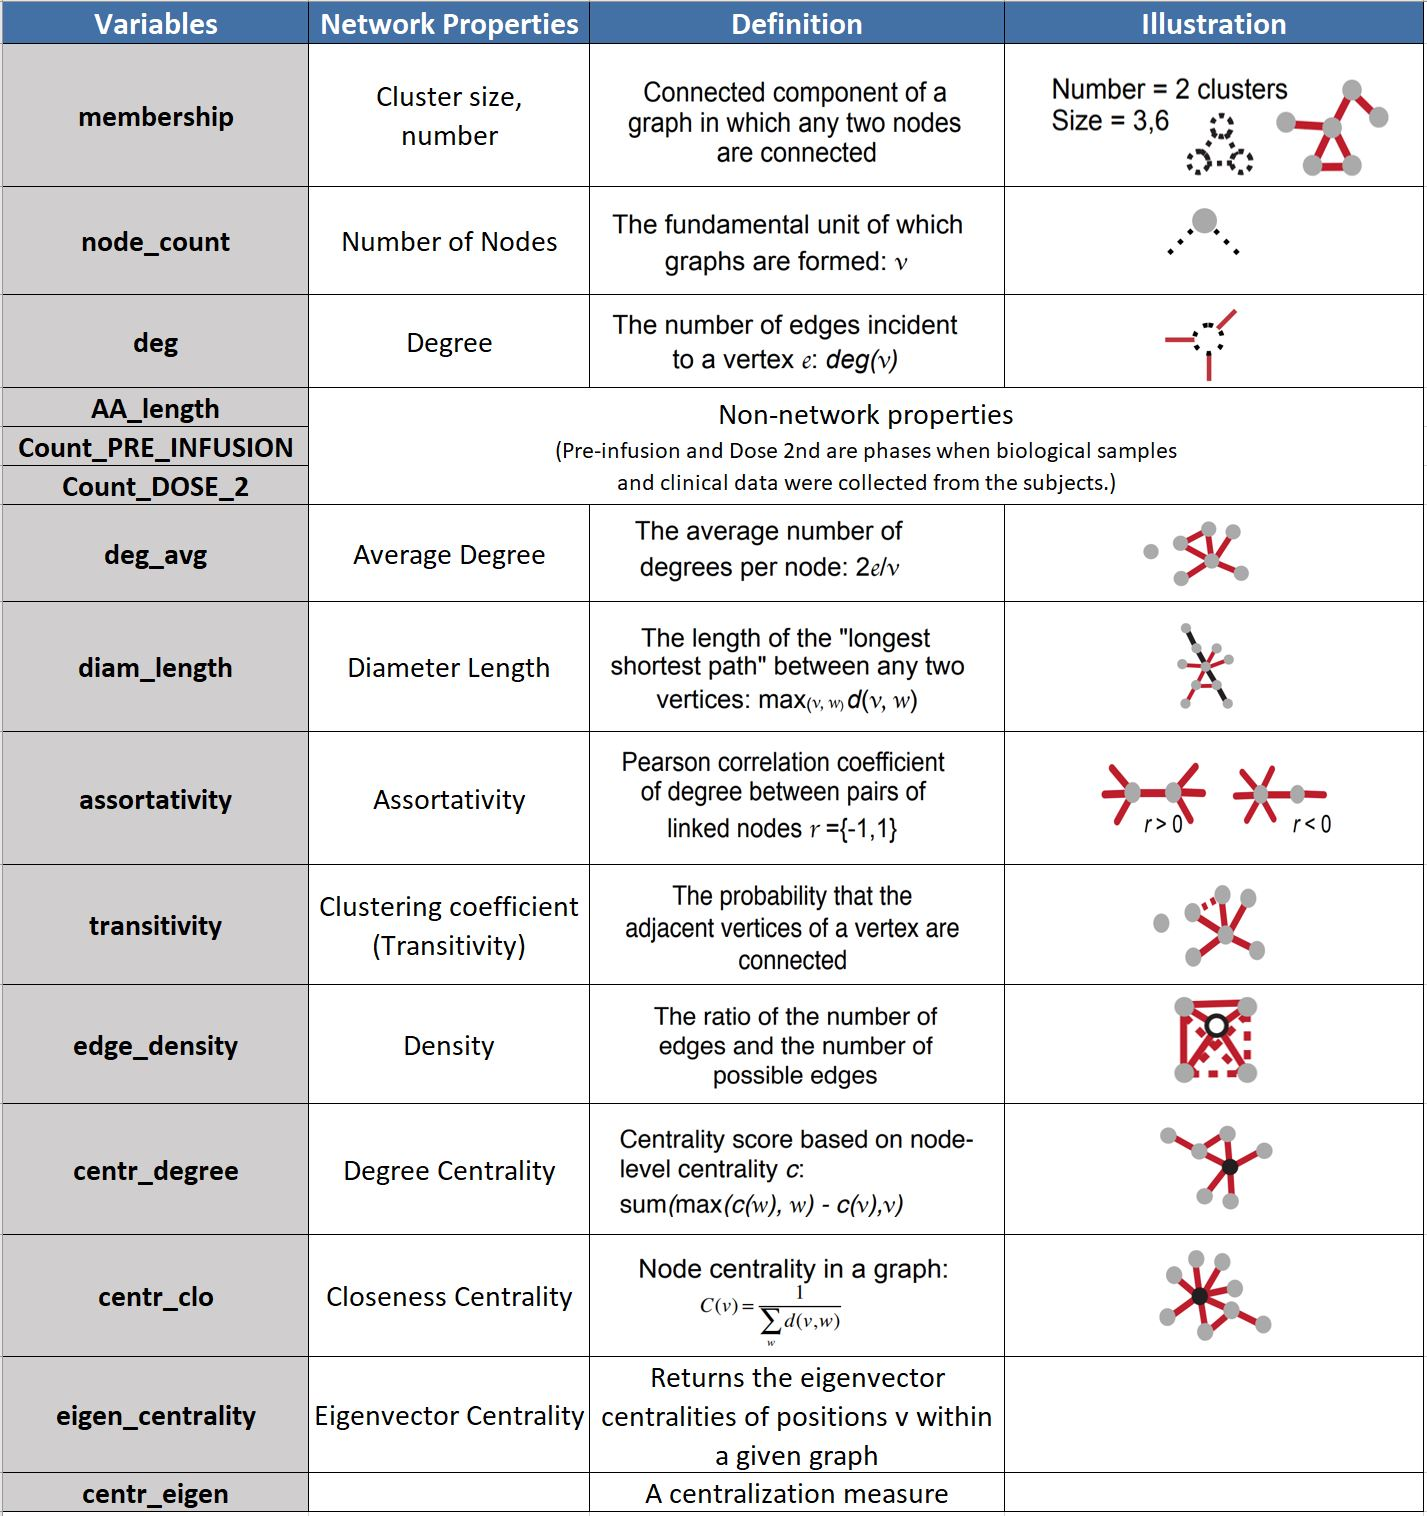
\includegraphics[scale=0.75]{NetworkProperties}
\caption{TCR network properties used for analysis (\cite{tcr_ntw}Miho \textit{et al.}, 2019).}
\label{fig:nw_prop}
\end{figure}

\section{Challenges}\label{sec:challenges}
The response variable, $OS\_mon$, has a single value for each of the 65 patients. We require the explanatory variables to be aligned similarly to make inferences. However, the TCR network data consists of a mix of global and local variables. The global variables are described by a single value, while the local variables are vectors of varying length. Since the TCR repertoire is constantly adapting to the health and the environmental factors of the patient, the network properties are continually shaping. Given any two patients the TCR repertoire is never the same. In fact, there is less than 20$\%$ overlap observed across the TCR repertoire for the same subject. This heterogeneous nature of the TCR repertoire and network properties makes it extremely difficult to perform statistical inference or machine learning directly between subjects. The heterogeneity issue also complicates the data simulation process required to perform the simulation study. Therefore, we require to develop ingenious ways to handle the TCR network data throughout our work and derive meaningful inferences.\par

\section{Contribution}\label{sec:contribution}
In this paper we proposed a strategy to extract features from the heterogeneous global\/local network properties. Reading through the distribution of the network properties using the real data, we collect some summary statistics. These derived summary statistics (referred to as the network features) largely consist of the Minimum, the $1^{st}$ Quartile $(Q_1)$, the Median, the Mean, the $3^{rd}$ Quartile $(Q_3)$ and the Maximum values. This technique is uniformly repeated for all the properties. Now the network properties are represented by aggregating these summary statistics (referred to as the feature blocks/groups). This approach helps us to sum up the TCR network properties for each patient and renders the data suitable for making statistical inferences.\par

We then apply the variable selection techniques like Lasso (\cite{tibshir}Tibshirani, 1996), Group Lasso , (\cite{grouporigin}Yuan and Lin, 2005), and Exclusive Lasso (\cite{exclusv_lasso}Zhou, Jin and Hoi, 2010) to prioritize the T-cell Receptor (TCR) network properties and to select the top network features. The technique of Group Lasso is applied to the feature blocks. As a virtue of this method we were able to identify the significant feature blocks. Next, we leveraged the Lasso and Exclusive Lasso techniques to identify the top performing network features (significant summary statistics) from these blocks. We observed a small coherence between the results. This could have resulted due to the small sample size (65 data rows). Variable selection methods generally use the cross-validation technique to render the optimal tuning parameter $\lambda$ that aids in shrinking and selecting the significant variables. Through this work we presented a comparison of how the cross-validation technique performs against a fairly new technique called the permutation-assisted tuning. This new technique uses a permutation copy of the original data set, with the intention of disrupting any correlation that exists among the explanatory variables and that between the explanatory variables and the response variable. This creates a data set with pseudo-variables that has the same dimensions as  the original data set. The final data is widened (predictor space is doubled) by augmenting both the original data set (using the true active variables) and the permutation copy (using the pseudo-variables). The modified data is then fed into the variable selection algorithms to identify a tuning parameter $\lambda$ such that the pseudo-variables are never selected. The permutation tuning technique is known to have lower false positives than the cross-validation technique. So far, the permutation assisted tuning has been used only on Lasso models. We add novelty in expanding its application to Group Lasso models and present how this technique can be used to identify the significant feature blocks. During this work we also deduced that the permutation assisted tuning method cannot be applied to Exclusive Lasso models. The Exclusive Lasso model bounded by its design selects at least one feature from every existing feature block. Hence, Exclusive Lasso will never converge to find a $\lambda$ value which can differentiate between the true variables and the pseudo-variables when using permutation tuning.\par

We proposed a procedure to simulate the network properties using the real data. The network property distributions gave us an insight to some of the correlations that existed among the explanatory variable. Using those correlation structure we first simulated a heterogeneous form of the TCR network data and then aggregated it using the summary statistics technique proposed earlier. The simulated data set gave us the flexibility to compare the model performances and ensured the soundness of the results using various performance measures like --- Sensitivity, False Discovery Rate, F1 score, Power, and Stability.\par

We provide the results of our analysis from the real data, where we are able to capture some of the significant network properties (feature blocks) and network features (summary statistics). In order to validate those results and compare between the different variable selection methods we perform the simulation study. In this section we present an alternative technique than GPUs to perform large-scale network data simulation. Analyzing the network properties, identifying the superficial dependencies and correlations guides us to simulate the network data. The simulated data is then fed into the variable selection models and performance measures like - Sensitivity, False Discovery Rate, F1 score, Power and Stability are computed. We make an interesting observation that the permutation assisted tuning method, used to derive the tuning parameter, outperforms the cross-validation technique when performing variable selection. We finally produce the larger set of significant network properties and the top network features that contribute in determining increase overall survival months in the patients.\par

